\documentclass[14pt, a4paper]{extarticle}
\usepackage{GOST}
\usepackage{array}
\usepackage{verbatim}
\usepackage[detect-all]{siunitx}
\usepackage{amsmath}
\usepackage{amssymb}
\usepackage[utf8]{inputenc}
\usepackage{hyperref}

\usepackage{ifthen}


\usepackage{tempora}


\makeatletter
\renewcommand\@biblabel[1]{#1.}
\makeatother

% Для листинга кода:
\usepackage{listings}
\lstset{ %
	language=python,                 % выбор языка для подсветки (здесь это С)
	basicstyle=\small\sffamily, % размер и начертание шрифта для подсветки кода
	numbers=left,               % где поставить нумерацию строк (слева\справа)
	numberstyle=\tiny,           % размер шрифта для номеров строк
	stepnumber=1,                   % размер шага между двумя номерами строк
	numbersep=5pt,                % как далеко отстоят номера строк от подсвечиваемого кода
	showspaces=false,            % показывать или нет пробелы специальными отступами
	showstringspaces=false,      % показывать или нет пробелы в строках
	showtabs=false,             % показывать или нет табуляцию в строках
	frame=single,              % рисовать рамку вокруг кода
	tabsize=2,                 % размер табуляции по умолчанию равен 2 пробелам
	captionpos=t,              % позиция заголовка вверху [t] или внизу [b] 
	breaklines=true,           % автоматически переносить строки (да\нет)
	breakatwhitespace=false, % переносить строки только если есть пробел
	escapeinside={\#*}{*)}   % если нужно добавить комментарии в коде
}


%для графиков
\usepackage{pgfplots}
\usepackage{filecontents}
\usetikzlibrary{datavisualization}
\usetikzlibrary{datavisualization.formats.functions}

\begin{document}
	
	\begin{table}[ht]
		\centering
		\begin{tabular}{|c|p{400pt}|} 
			\hline
			\begin{tabular}[c]{@{}c@{}} 
\includegraphics[scale=1]{baum.jpg} \\\end{tabular} &
			\footnotesize\begin{tabular}[c]{@{}c@{}}\textbf{Министерство~науки~и~высшего~образования~Российской~Федерации}\\\textbf{Федеральное~государственное~бюджетное~образовательное~учреждение}\\\textbf{~высшего~образования}\\\textbf{«Московский~государственный~технический~университет}\\\textbf{имени~Н.Э.~Баумана}\\\textbf{(национальный~исследовательский~университет)»}\\\textbf{(МГТУ~им.~Н.Э.~Баумана)}\\\end{tabular}  \\
			\hline
		\end{tabular}
	\end{table}
	\noindent\rule{\textwidth}{4pt}
	\noindent\rule[14pt]{\textwidth}{1pt}
	\hfill 
	\noindent
	\makebox{ФАКУЛЬТЕТ~}%
	\makebox[\textwidth][l]{\underline{~«Информатика и системы управления»~~~~~~~~~~~~~~~~~~~~~~~~~~~~~~~~~}}%
	\\
	\noindent
	\makebox{КАФЕДРА~}%
	\makebox[\textwidth][l]{\underline{~«Программное обеспечение ЭВМ и информационные технологии»~}}%
	
	
	\begin{center}
		\vspace{1.5cm}
		{\bf\huge Отчёт\par}
		{\bf\Large по лабораторной работе № 3\par}
		\vspace{0.7cm}
	\end{center}
	
	
	\noindent
	\makebox{\large{\bf Название:}~~~}
	\makebox[\textwidth][l]{\large\underline{Исследование псевдослучайных чисел~~~~~~~~}}
	
	\noindent
	\makebox{\large{\bf Дисциплина:}~~~}
	\makebox[\textwidth][l]{\large\underline{~Моделирование~~~~~~~~~~~~~~~~~~~~~~~~~~}}\\
	
	\vspace{1.5cm}
	\noindent
	\begin{tabular}{l c c c c c}
		Студент      & ~ИУ7-75Б~               & \hspace{2.5cm} & \hspace{2cm}                 & &  Д.В. 
		Сусликов \\\cline{2-2}\cline{4-4} \cline{6-6} 
		\hspace{3cm} & {\footnotesize(Группа)} &                & {\footnotesize(Подпись, дата)} & & {\footnotesize(И.О. Фамилия)}
	\end{tabular}
	
	\noindent
	\begin{tabular}{l c c c c}
		Преподаватель & \hspace{5cm}   & \hspace{2cm}                 & & ~~~~~~И.В. Рудаков~~~~~~\\\cline{3-3} \cline{5-5} 
		\hspace{3cm}  &                & {\footnotesize(Подпись, дата)} & & {\footnotesize(И.О. Фамилия)}
	\end{tabular}
	
	\vspace{0.6cm}
	\begin{center}	
		\vfill
		\large \textit {Москва, 2021}
	\end{center}
	
	\thispagestyle {empty}
	\pagebreak
	
	% СОДЕРЖАНИЕ 
	\clearpage
	\tableofcontents
		
	% ВВЕДЕНИЕ
	\clearpage
	\section*{Задание}
	\addcontentsline{toc}{section}{Задание}
	Изучить методы генерирования псевдослучайных чисел, а также критерии оценки случайности последовательности. Реализовать критерий оценки случайной последовательности. Сравнить результаты работы данного критерия на одноразрядных, двухразрядных и трехразрядных последовательностях целых чисел. Последовательности получать алгоритмическим и табличным способами.
	
	\clearpage
	\section*{Теория}
	\addcontentsline{toc}{section}{Теория}
	
	\textbf{Псевдослучайная последовательность (ПСП)} — последовательность
	чисел, которая была вычислена по некоторому правилу, но имеет свойства
	случайной последовательности чисел в рамках решаемой задачи.\par
	
	\textbf{Табличный способ генерация ПСП}\par
	Табличные генераторы в качестве источника случайных чисел используют заранее подготовленные таблицы, содержащие проверенные некоррелированные числа. Недостатки такого способа являются использование внешнего ресурса для хранения чисел и период, ограниченный размером таблицы.\par
	
	\textbf{Алгоритмический способ генерация ПСП}\par
	Алгоритмические генераторы случайных чисел для получения следующего псевдослучайного числа используют некоторое математическое правило, например, линейный конгруэнтный метод. В данном работе последовательность генерируется при помощи формулы: 
	\begin{equation}
		X_{n+1} = (aX_n + c) mod \text{ }m
	\end{equation}
	

	\textbf{Критерий оценки случайности последовательности}\par
	Для выполнения работы был выбран критерий «хи квадрат ».
	\begin{equation*}
		V = \frac{1}{n} \sum_{s=1}^{k}(\frac{Y_s^2}{p_s}) - n,
	\end{equation*}
	 Это один из
	самых известных статистических критериев, также это основной метод,
	используемый в сочетании с другими критериями. 

	\clearpage
	\section*{Примеры}
	Смотря на примеры работы программы для последовательности чисел в количестве 10000, сгенерированных линейным
	конгруэнтным и табличным методами, можно сделать вывод, что лучше себя в точности показал табличный метод.
	\addcontentsline{toc}{section}{Примеры}
	
	\begin{figure}[h!]
		\centering{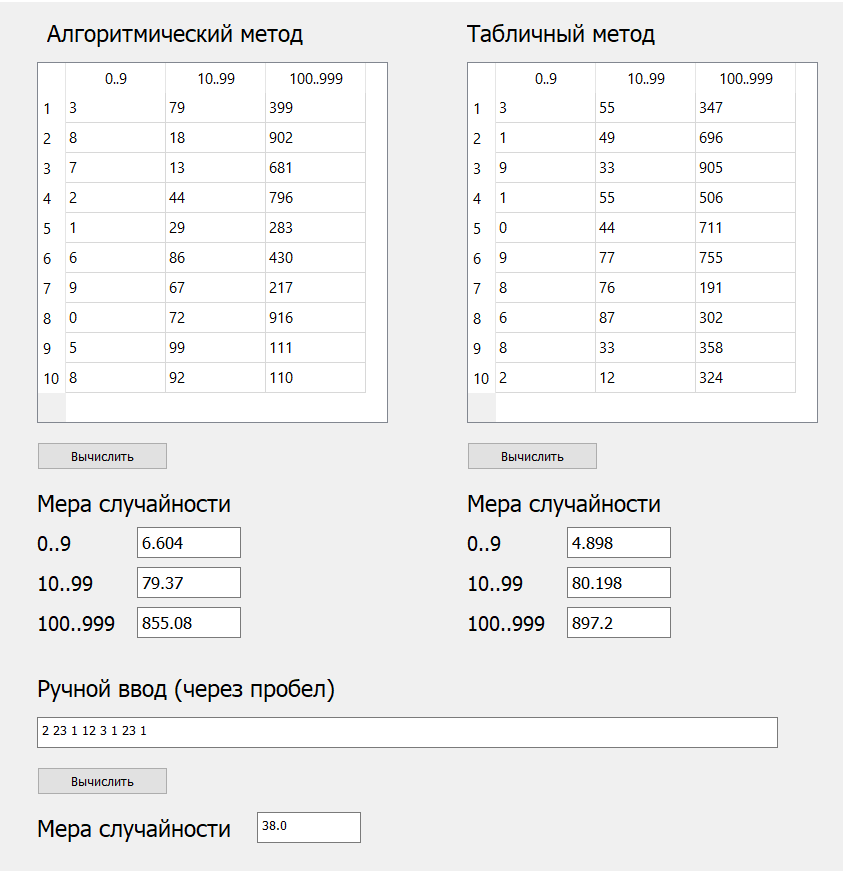
\includegraphics[scale=0.9]{source/1}}
		\centering\caption{Пример 1}
	\end{figure}
	\newpage
	

	\begin{figure}[h!]
		\centering{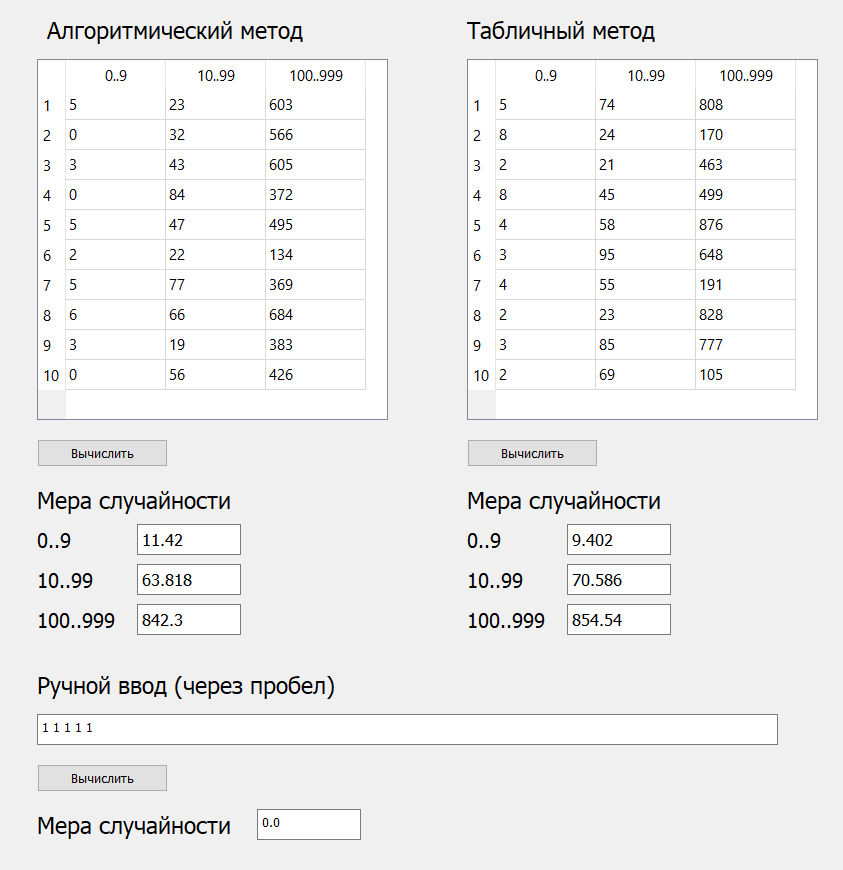
\includegraphics[scale=0.9]{source/2}}
		\centering\caption{Пример 2}
	\end{figure}
	\newpage
	
	\begin{figure}[h!]
		\centering{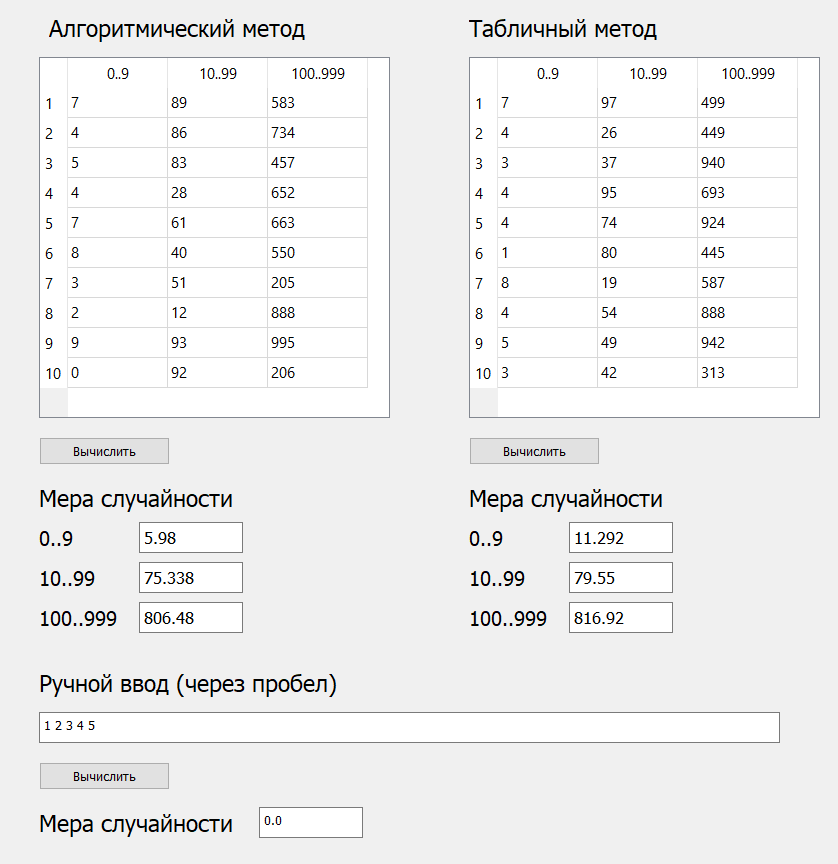
\includegraphics[scale=0.9]{source/3}}
		\centering\caption{Пример 3}
	\end{figure}

	\clearpage
	\section*{Листинги}
	\addcontentsline{toc}{section}{Листинги}
	
	\begin{lstlisting}[caption=lab3.py]
		import sys
		from PyQt5 import QtWidgets
		from PyQt5 import uic, QtWidgets, QtGui
		from PyQt5.QtWidgets import QApplication, QWidget, QListWidgetItem,  QTableWidgetItem, QMessageBox
		import design
		from itertools import islice
		
		COUNT = 10000
		
		class App(QtWidgets.QMainWindow, design.Ui_MainWindow):
			def __init__(self):
				self.current = 10
				self.m = 2.**32
				self.a = 1664525
				self.c = 1013904223
				self.count = 1
			
			super().__init__()
				self.setupUi(self)
				self.initUI()    
				
				self.setFixedSize(858, 875) 
			
			def initUI(self):
				self.calcAlgBtn.clicked.connect(self.calcAlgBtnPushed)
				self.calcTableBtn.clicked.connect(self.calcTableBtnPushed)
				self.calcManualBtn.clicked.connect(self.calcManualBtnPushed)
				
			def get_number(self, low=0, high=100):
				self.current = (self.a * self.current + self.c) % self.m
				result = int(low + self.current % (high - low))
				return result
			
			
			def calcAlgBtnPushed(self):
				one_alg, two_alg, three_alg = self.alg_rand()
			
				for i in range(10):
					self.tableAlg.setItem(i, 0, QTableWidgetItem(str(one_alg[10*(self.count-1):10*self.count][i])))
					self.tableAlg.setItem(i, 1, QTableWidgetItem(str(two_alg[10*(self.count-1):10*self.count][i])))
					self.tableAlg.setItem(i, 2, QTableWidgetItem(str(three_alg[10*(self.count-1):10*self.count][i])))
					
				self.measureAlg1.clear()
				self.measureAlg2.clear()
				self.measureAlg3.clear()
				self.measureAlg1.setText(str(round(self.calc_hi(one_alg, 10000, 0, 10), 3)))
				self.measureAlg2.setText(str(round(self.calc_hi(two_alg, 10000, 10, 100), 3)))
				self.measureAlg3.setText(str(round(self.calc_hi(three_alg, 10000, 100, 1000), 3)))
					
					self.count += 1
			
			def calcTableBtnPushed(self):
				one_tbl, two_tbl, three_tbl = self.table_rand()

				for i in range(10):
					self.tableTable.setItem(i, 0, QTableWidgetItem(str(one_tbl[:10][i])))
					self.tableTable.setItem(i, 1, QTableWidgetItem(str(two_tbl[:10][i])))
					self.tableTable.setItem(i, 2, QTableWidgetItem(str(three_tbl[:10][i])))
	
				self.measureTable1.clear()
				self.measureTable2.clear()
				self.measureTable3.clear()
				self.measureTable1.setText(str(round(self.calc_hi(one_tbl, 10000, 0, 10), 3)))
				self.measureTable2.setText(str(round(self.calc_hi(two_tbl, 10000, 10, 100), 3)))
				self.measureTable3.setText(str(round(self.calc_hi(three_tbl, 10000, 100, 1000), 3)))
				
				self.count += 1
			
			def table_rand(self):
				numbers = set()
				with open('numbers.txt') as file: 
					line_num = 0
					lines = islice(file, line_num, None)
					for l in lines:
						numbers.update(set(l.split(" ")[1:-1]))
						line_num += 1
						if len(numbers) >= 3* COUNT + 1:
							break
					numbers.remove("") 
					numbers = list(numbers)[:3*COUNT]
				one_digit = [int(i)%10 for i in numbers[:COUNT]]
				two_digits = [int(i)%90 + 10 for i in numbers[COUNT:COUNT * 2]]
				three_digits = [int(i)%900 + 100 for i in numbers[COUNT*2:3*COUNT]]
				return one_digit, two_digits, three_digits
			
			def alg_rand(self):
				one_digit = [self.get_number(0, 10) for i in range(COUNT)]
				two_digits = [self.get_number(10, 100) for i in range(COUNT)]
				three_digits = [self.get_number(100, 1000) for i in range(COUNT)]
				return  one_digit, two_digits, three_digits
			
			def calc_hi(self, arr, n, start, end): 
				tab = [0 for i in range(start + end)]
			
				for i in range(n):
					tab[arr[i]] += 1
				s = 0
				
				for i in tab:
					s += i * i				
				return s * (end-start) / n - n 
			
			def calcManualBtnPushed(self):
				nums = self.manualText.toPlainText().split()
				for i in range(len(nums)):
				nums[i] = int(nums[i])
				
				hi = self.calc_hi(nums, len(nums), min(nums), max(nums)+1)
				self.measureManual.setText(str(round(hi, 3)))
			
		def main():
			app = QtWidgets.QApplication(sys.argv)
			window = App()
			window.show()
			app.exec_()
		
		if __name__ == '__main__':
			main()		
	\end{lstlisting}	
\end{document}